\documentclass[procedia]{easychair}

% This provides the \BibTeX macro
\usepackage{doc}
\usepackage{makeidx}
% If you plan on including some algorithm specification, we recommend
% the below package. Read more details on the custom options of the
% package documentation.
%
\usepackage{algorithm2e}

\def\procediaConference{99th Conference on Topics of
	Superb Significance (COOL 2014)}

%% Front Matter
%%
% Regular title as in the article class.
%
\title{Parallel Simulation of Adaptive Random Boolean Networks}

% \titlerunning{} has to be set to either the main title or its shorter
% version for the running heads. When processed by
% EasyChair, this command is mandatory: a document without \titlerunning
% will be rejected by EasyChair

\titlerunning{Parallel Simulation of Adaptive RBNs}

% Authors are joined by \and. Their affiliations are given by \inst, which indexes into the list
% defined using \institute
%
\author{
	Kirill Kuvshinov\inst{1}
	\and
	Klavdiya Bochenina\inst{1}
	\and
	Piotr Gorsky\inst{2}
	\and
	Janusz Holyst\inst{1}\inst{2}
}

% Institutes for affiliations are also joined by \and,
\institute{
	ITMO University, St. Petersburg, Russian Federation
	\and
	Warsaw University of Technology, Warsaw, Poland
}
%  \authorrunning{} has to be set for the shorter version of the authors' names;
% otherwise a warning will be rendered in the running heads. When processed by
% EasyChair, this command is mandatory: a document without \authorrunning
% will be rejected by EasyChair

\authorrunning{Kuvshinov, Bochenina, Gorsky, Holyst}

\begin{document}
	
	\maketitle
	
	\keywords{adaptive random boolean networks, GPGPU algorithm, parallel simulation}
	
	\begin{abstract}
		A random boolean network (RBN) is a generic model of interactions between entities with binary states that has applications in different fields. As real-world systems often operate on the border between order and chaos, the algorithms of RBN's transition to a critical state are of particular interest. Adaptive RBNs can evolve towards a critical state by rewiring nodes according to their states on the attractor. Numerical simulation of adaptive RBN larger than several dozens of nodes is computationally hard due to the enormous growth of the lengths of attractors and transient periods. In this paper, we propose GPGPU algorithm for parallel simulation of adaptive RBNs with modified activity-dependent rewiring rule which can be used with any sequential algorithm for attractor's search. In the experimental part of the study, we investigate the performance of parallel implementation and the influence of parameters of the algorithm on the speed of convergence to a steady state. 
	\end{abstract}
	
	
	%------------------------------------------------------------------------------
	\section{Introduction}
	\label{sect:introduction}
	
	One of goals of complex networks analysis is a better understanding, description and prediction of the behavior of real-world systems. A starting point are usually simplified models that have few parameters and driven by random dynamics. The example of such a model is a random Boolean network (RBN) \cite{gershenson04,drossel2008random,cheng2011random,aldana2003boolean}. 
	
	RBNs were initially introduced to describe gene regulatory networks \cite{kauffman1969metabolic,kauffman2004ensemble}. But as RBNs are generic they were also applied to other fields, e.g. neural networks and social networks \cite{drossel2008random}.
	
	An RBN is a directed network consisting of ${N}$ nodes. A node $i$ ($i=1, ..., N$) has three attributes: (a) a Boolean state $\sigma_i(t)\in \{0,1\}$, (b) a sequence $\boldsymbol{N_i}$ containing all nodes ($\sigma_{i_1}, \sigma_{i_2}, \ldots, \sigma_{i_{|\boldsymbol{N_i}|}}$) having a connection to the node $i$ and (c) a randomly chosen Boolean function $f_i: \{0,1\}^{|N_i|} \rightarrow \{0,1\}$. 
	Note that we assume a network with no loops, that is  $i \not\in \boldsymbol{N_i}$. 
	Arguments of the function $f_i$ are states of the nodes from $\boldsymbol{N_i}$. Boolean functions determine nodes' states in the next time step:
	\begin{equation}
	\sigma_i(t+1) = f_i(\sigma_{i_1}(t), \sigma_{i_2}(t), \ldots, \sigma_{i_{|\boldsymbol{N_i}|}}(t)),
	\label{eq:update}
	\end{equation}
	Each Boolean function is randomly chosen. It means that a node $n_i$ has $2^{2^{|N_i|}}$ possible different Boolean functions and one of them is chosen at random.
	%(During network evolution nodes update their states with their Boolean functions. )
	Taking also into consideration all network topologies, the size of the network ensemble is enormous. That is why RBNs are generic and despite their simplicity they can model many complex systems \cite{drossel2008random}. 
	
	We assume all the nodes are updated according to the Eq. (\ref{eq:update}) at the same time. Let $\boldsymbol{S}(t)=\{\sigma_1, \sigma_2, \ldots, \sigma_N\}$ define a state of the whole network. 
	Having $N$ nodes in the network, network state space is $2^N$-dimensional. It can be huge, but it is finite. The update rule (\ref{eq:update}) is deterministic, thus after a number of transient network states, the system will eventually reach an attractor (i.e. a periodic orbit of network state $\boldsymbol{S}(t)$). 
	
	As RBNs are applied to model biological structures, it is interesting to study the evolution of RBNs. Core of the evolution process is a constant searching for \footnote{Tu sie nie zgadzam, ze powinno być of. Istnieja 2 zwroty: 'search for' oraz 'in search of'. Ten drugi znaczy 'w poszukiwaniu'.} the most optimal configuration \cite{aldana2003boolean,sole1996extinction,zimmermann2004coevolution}. 
	An RBN modification that incorporates system evolution is {\it adaptive} RBN (ARBN) \cite{mlb,soc,haruna14relationship,Gorski2016}. 
	In RBNs nodes can be divided into two groups of active and frozen nodes. Nodes of the former group change their state during network attractor. On the other hand, the frozen nodes keep their state. 
	The basis of ARBN is a natural idea that overactive nodes should be quietened down and underactive (frozen) ones should be stimulated. This concept is included in an activity-dependent rewiring rule (ADRR) \cite{bornholdt2000topological}, which is as follows: 
	if the node’s mean state $<\sigma_i>$ during the network attractor is $0$ or $1$, then this node
	is considered to be frozen and one new incoming edge is
	added to this node. Otherwise, this node is considered to be active and one of
	its incoming edges is randomly chosen and deleted.
	
	A single simulation of ARBN evolution consists of an a priori-defined number of epochs. In each epoch the network attractor is found (evolution of nodes' states) and incoming connections of randomly chosen node are updated according to the ADRR (evolution of network structure). 
	In the simulation results it is observed \cite{mlb,Gorski2016}, that after a number of transient epochs, the system reaches a dynamical equilibrium and oscillates around steady-state levels of measured values (e.g. mean connectivity). 
	
	In this paper, we perform ARBN simulations for larger networks with up to $1~000$ nodes. 
	In such structures the difficulty is in finding the attractor because transient and attractor lengths grow quickly with network size. 
	In previous work there have been only few results with such network sizes. In original paper \cite{mlb} the full model analysis is for the network of size up to $400$ nodes\footnote{TODO: Later it might be emphasized that LiuBassler results must have skipped most (significant number) of the attractors.}. 
	In our previous work, where we analyze modular Boolean networks with separate ARBNs connected by a number of interlinks \cite{Gorski2016}, the studied maximal network size is $80$ nodes. 
	Here, we do not include modularity into ARBN model. 
	This research is a step towards large scale simulations of modular ARBNs \cite{Gorski2016}. To investigate large ARBNs, we design a parallel algorithm for simulation of ARBN's evolution and combine it with several algorithmic improvements.
	
	The remaining part of the paper is organized as follows. Section 2 gives an overview of a related work on algorithmics of RBN modeling. Section 3 presents a description of algorithms and techniques which were used to speed up simulations (including an algorithm for parallel simulation of adaptive RBNs). Section 4 (an experimental investigation) has two-fold purpose: (i) to study the performance of the parallel algorithm and the influence of proposed modifications on simulation results, and (ii) to study the dynamics of evolution of non-modular ARBNs up to 1000 nodes.

	%------------------------------------------------------------------------------
	\section{Related Work}
	\label{sect:related-work}
	In recent years, a variety of RBNs has been extensively studied by the means of computer simulation. Basically, an initial topology, a set of boolean functions and an updating scheme (synchronous or asynchronous) \cite{gershenson04} are fixed. In contrast, adaptive RBN can evolve by changing links and/or boolean functions of nodes. Bornholdt and Sneppen in \cite{bornholdt1998neutral} introduced an algorithm for RBN's evolution under the constraint of continuity. In the algorithm, a degree of a randomly chosen node is modified only when a network with this modification reaches the same attractor as the mother system did. Paczuski, Bassler and Corral in \cite{paczuski2000self} consider nodes of RBN as competing agents in a market. The evolution of network is maintained by a random change of the poorest player's strategy at each epoch of simulation. ADDR as a mechanism for transition of RBN to a critical state was proposed in \cite{bornholdt2000topological} and then extended in \cite{mlb} for annealed and quenched versions of a model. Both in  \cite{bornholdt2000topological} and \cite{mlb} ADDR changes a single randomly chosen node per iteration according to its average state on the attractor; the difference is that in \cite{mlb} boolean functions of nodes can also be changed at the end of the epoch. 
	
	Simulation of a single epoch for adaptive RBN consists of two steps, search for an attractor and modification of a network according to chosen rules. Depending on the goal of simulation, it could be necessary to find a single attractor for a given initial state or all the attractors of a system. Zhang et. al. in \cite{zhang2007algorithms} propose algorithms to find singleton attractors of RBN using gene ordering. To find a single attractor of an arbitrary length, there are two main algorithms: Knuth's algorithm \cite{knuth1981art} (the example of its usage for RBN's simulation can be found in \cite{bhattacharjya1996median}) and the algorithm described in \cite{mlb} (we denote it as Liu-Bassler). We include the brief description of these algorithms in Section 3 of this paper as they serve as a basis for our parallel algorithm. The second category includes algorithms to find all attractors for a given network. These algorithms usually reformulate basic task as binary decision diagrams, satisfiability (SAT) or aggregation problems. For the asynchronous update mode, there was proposed an approach based on an exhaustive enumeration of subspaces of a network space implemented in Inet software package \cite{berntenis2013detection}. Some of the algorithms of this type allow parallel implementation (e.g. \cite{guo2014parallel}). Parallelization is performed by calculating different attractors (or sets of attractors) for the same network on different processors, and is not appropriate for ADDR having data dependency between epochs. 
	
	Another way to speed up a simulation of RBN is to choose appropriate data types and data structures to keep a network, and use efficient implementations of nodes' update function. The example of this approach can be found in \cite{hawick2007simulating} where authors explore high-performance data structures and algorithms for large-scale simulations of RBNs for D programming language. They examine the memory complexity and the performance of the RBN simulation code for 256 iterations (for networks up to 2,5 million nodes) and for 8 iterations (for networks up to 20,5 million nodes). However, the applicability of the results for ARBNs is restricted as a simulation of an evolution of large networks becomes computationally intractable because of an enormous number of iterations rather than a large execution time of a single iteration.
	
	Due to the exponential slowing down by long attractor periods for initial connectivity $K_{ini} \geq 2$, usually it is necessary to put the restrictions on a maximum number of iterations to be examined during a single search for attractor (it is denoted as $T_{max}$). In \cite{bornholdt2000topological}, authors use $T_{max} = 1000$ which allows them to study networks up to 1024 nodes. In \cite{mlb}, $T_{max}$ is set up to 100 000, and the maximum size of a studied network is equal to 400 nodes. Increase of a size of a network with fixed $T_{max}$ leads to skipping a significant number of the attractors. However, authors of \cite{bornholdt2000topological} and \cite{mlb} do not consider a percentage of attractors found, and how the results of simulation are influenced by skipped attractors.
	

	%------------------------------------------------------------------------------
	\section{Algorithms to Speed up Simulation of ARBNs}
	\label{sect:algorithm}
	
	
	Modeling the evolution of ARBN larger than several dozens of nodes is hampered by a significant growth of transient and attractor lengths. This growth extremely prolongs the time of a repeated calculation of nodes' states during search for an attractor (which is the most time consuming part of a modeling). To speed up modeling for large ARBNs, we propose to combine algorithms and techniques described in this Section. We use existing sequential algorithms for attractor's search with a limitation on a maximum number of iterations as a basis of the parallel algorithm, and extend ADDR to support larger number of nodes to be rewired. 
	
	\paragraph{I. Sequential heuristics for attractor's search.} The naive implementation of an algorithm for attractor's search is to compare a current state $\mathbf{S}(t)$ to all the previous states at each iteration. This requires $O(l^2)$ time and $O(l)$ memory where $l$ is a sum of attractor and transient lengths. 	
	To speed up searching for attractors in comparison with the naive implementation a number of sequential heuristics have been proposed. These algorithms do not perform the exhaustive comparisons of states. Here we briefly describe and discuss two sequential algorithms which have been used in previous studies on ARBN \cite{mlb,Gorski2016}. We also use them as basic algorithms for a parallel algorithm introduced in this paper.
	
	\paragraph{Liu-Bassler algorithm.} This is the algorithm that was used in the original paper introducing Adaptive RBNs \cite{mlb}.  It is based on a set of checkpoints $\mathbf{T} = \{T_0, T_1, T_2, ... T_n\}$. If at some time point $t$ current state $\mathbf{S}(t)$ equals to the state at the checkpoint $\mathbf{S}(T_i)$, an attractor is considered to be found, and some nodes get rewired according to the ADRR presented above. If the program reaches the next checkpoint (except the last one), and $\mathbf{S}(t) \neq \mathbf{S}(T_i)$ $ \forall t \in [T_i, T_{i+1})$, all the information gathered between the checkpoints is discarded as it most probably corresponds to a transient period rather than the attractor, and $T_{i+1}$ becomes the new checkpoint. The longest attractor that can be found using this algorithm equals to the maximum distance between the checkpoints. However, if the distance between the checkpoints is too large, more state updates then necessary are performed. Thus, the values of the checkpoints are crucial to the overall algorithm performance and correctness.
	 
	\paragraph{Knuth algorithm.} (The description of Knuth algorithm)

\paragraph{II. Updating states of nodes in parallel.} Another way to reduce an execution time of modeling is to parallelize calculations of nodes' states at a particular iteration. In this study, we propose a GPGPU algorithm which speeds up sequential heuristics of type (I). As it does not influence the logic of a search, this algorithm can be used in a combination with any sequential heuristic. The main idea of the algorithm is to update states of different nodes in a network in parallel on distinct Graphic Processor Units (GPUs). More formal description is presented in Algorithm \ref{algo:gpu}.

	\begin{algorithm}[ht!]
		\label{algo:gpu}
		GenerateNetwork()\;
		\While{ epoch $<$ epochsCount }
		{
			$gpuNetwork \leftarrow$ ConvertNetworkToGpuRepresentation()\;
			ZeroInitialize($stateSum$)\;
			CopyToGpu($gpuNetwork$, $currentState$, $stateSum$)\;
			\While{attractor not found}
			{ 	
				UpdateStateOnGpu($currentState$, $stateSum$)\;
			}
			CopyFromGpu($stateSum$)\;
			$nodesToRewire \leftarrow$ ChooseRandomNodes($N_{rew}$)\;
			ActivityDependentRewiring($nodesToRewire$, $stateSum$)\;
			epoch = epoch + 1\;
		}
		\caption{GPGPU algorithm for ARBN simulation}
	\end{algorithm}

	\paragraph{} The performance of the GPU implementation highly depends on the Boolean network representation it uses. Since a node with inputs \(\mathbf{N_i}\) has \(2^{|\mathbf{N_i}|}\) possible combinations of inputs' state, it is a common approach to store a Boolean function of the node as \(1 \times 2^{|\mathbf{N_i}|}\) vector \(\mathbf{b_i}\). We can represent these vectors as \(N \times 2^{\max{|\mathbf{N_i}|}}\) matrix \(B\).
	
	Having Boolean functions stored this way, one can obtain the next state of the network using one sparse matrix-vector multiplication (Eq. (\ref{eq:spmv})) and one gather operation (Eq. (\ref{eq:gather})).
	
	\begin{equation}
	\label{eq:spmv}
		\mathbf{v} = A \times \mathbf{S}(t)
	\end{equation}
	\begin{equation}
	\label{eq:gather}
		\sigma_i(t+1) = B_{i, \mathbf{v}_i}
	\end{equation}
	
	These operations are well-studied and efficient algorithms for GPGPU exist \cite{bell2008efficient}\cite{he2007efficient}.
	
	The matrix \(A\) is constructed as defined in Eq. (\ref{eq:matrix}), (\ref{eq:matrix_ii}). The special case in Eq. (\ref{eq:matrix_ii}) ensures that nodes with no in-connections do not change their states.
	
	\begin{equation}
		\label{eq:matrix}
		A_{ij} = \begin{cases}
			2^k, & \mbox{ if } i\mbox{ is a } k \mbox{-th input of } j \\
			0, & \mbox{otherwise}
		\end{cases} \mbox{  } \forall i \neq j
	\end{equation}
	\begin{equation}
	\label{eq:matrix_ii}
	A_{ii} = \begin{cases}
		1, & \mbox{if } |\mathbf{N}_i|=0\\
		0, & \mbox{otherwise}
		\end{cases}
	\end{equation}
	
	 Such representation supports different SpMV algorithms. These algorithms mainly aim at maximizing memory throughput and data locality, thus reducing the overall GPU kernel execution time. We chose compressed sparse-row (CSR) matrix storage format and implemented an SpMV kernel as described in \cite{bell2008efficient}, as it shows the best performance on unstructured matrices.
	
	However, the lenghts of attractors and transient periods grow faster than a power law[][] when the size of the network increases. This leads to a proportional growth of state updates one has to perform to find an attractor. The number of state updates turned out to be more important to the algorithm performance due to the lags between GPU kernel launches and the need to transfer data back from the GPU. 
	
	\paragraph{III. Limiting the number of state updates.} For RBN in a critical state, lengths of attractors and transients tend to have a power-law distribution with an exponent of -1 \cite{greil2009attractor}. This implies that a number of attractors with a given length is in inverse proportion to that length, i.e. a major part of attractors has comparatively small lengths. During evolution of ARBN, the goal is to find an attractor at each epoch, and then modify the topology of a network according to a state of a randomly chosen node on the attractor. While searching for an attractor, one can add a limitation on a maximum number of iterations which will be examined for a single epoch. In Liu-Bassler algorithm this limitation is a part of the algorithm itself (as it has predefined checkpoints) while in Knuth's algorithm is can be added artificially. The logic behind this approach is that lengthy attractors are rare, so a limitation can be set in a way that will not significantly influence the dynamic of convergence to a steady state. In this study we address the question: to what extent such limiting influence the qualitative results of simulation? In other words, we study how the results of ARBN evolution will differ if we eliminate from consideration a part of lengthy attractors (extending the results which were reported in \cite{Gorski2016}).
	\paragraph{IV. Rewiring different number of nodes per epoch.} I (heuristics for attractor's search), II (parallel algorithm of updating the states) and III (limiting the number of state updates) are aimed to reduce an execution time of a single epoch. The total execution time is equal to the summation of times for all epochs, and the total number of epochs should be sufficient to reach the steady state. Therefore, another way to speed up the modeling process is to reduce a number of epochs which is required to achieve steady state. In this paper, we propose to perform it by a modification of ADRR intoduced in \cite{mlb}. Instead of rewiring a single node per epoch, we suggest to use several nodes as it could speed up the convergence to a steady state (especially for large networks) and, as a result, significantly decrease total time of simulation.
	

	
	%------------------------------------------------------------------------------
	\section{Experimental Study}
	\label{sect:experimental-study}
	
The modified algorithm of ARBN evolution consists of a set of consecutive epochs. In each epoch the network attractor is found and $N_{rew}$ nodes are rewired according to the modified ADRR. The maximum length of attractors $\mu_{max}$ is limited ether by predefined checkpoints in Liu-Bassler algorithm, or artificially in Knuth's algorithm in order to speed up the computations as described in Section \ref{sect:algorithm}. Due to this limitation only a fraction $R$ of the attractors is found. During the evolution process the system reaches a dynamical equilibrium, which can be observed by measuring network's mean in-degree connectivity $K$, defined in Eq. \ref{eq:connectivity}. As the network evolves, $K$ tends to some steady-state value $K_{ss}$.
	
	
	\begin{equation}
	\label{eq:connectivity}
		K = N^{-1} \sum_{i=1}^{N} {|\mathbf{N}_i|}
	\end{equation}
	
	Intuitively, Liu-Bassler algorithm of attractor's search would have shown better performance than the Knuth's one, as the latter requires at least $3 \mu$ state updates to find an attractor of length $\mu$. But in order to use Liu-Bassler algorithm one needs to choose the checkpoints correctly, which requires an a-priori knowledge of attractor and transient period distributions. This distribution depends on a network size, connectivity and structure (e. g. modular networks tend to have longer (shorter?) attractors than non-modular ones [ref]). We obtained an empirical distribution of attractor and transient lengths for different kinds of networks in our preliminary experiments with Knuth's algorithm. The checkpoints $T=[100, 200, 1000, 2000, ... \mu_{max}, 2 \mu_{max}]$ seem to be the best trade-off between the number of state updates and the percentage of attractors found. However, with these checkpoints the difference in the number of state updates between the two algorithms is negligible. We used Knuth's algorithm in our future experiments, as it is more general and requires no a-priori knowledge of the network's behaviour.
	
	Both algorithms were implemented using C++ programming language. The implementation is cross-platform and requires a GPU with CUDA compute capability at least 1.2. The representation of RBNs' state update function defined in Eq. \ref{eq:spmv}, \ref{eq:gather} allows for experimenting with different SpMV algorithms. These algorithms mainly aim at maximizing memory throughput and data locality, thus reducing the overall GPU kernel execution time. We chose compressed sparse-row (CSR) matrix storage format and implemented an sparse matrix-vector multiplication kernel as described in \cite{bell2008efficient}, as it shows the best performance on unstructured matrices.
	
	To test the applicability of the approaches presented in Section \ref{sect:algorithm}, a set of experiments was performed. The experiments were conducted on a cluster consisting of 20 nodes with NVidia GeForce GT 640 graphic cards. In this study we considered only the networks with initial in-degree connectivity $K_{ini}=2$. The results were averaged over 10 realizations of the evolution process.
	
	\paragraph{Speedup obtained by GPU acceleration.} We measured the execution times of both sequential and parallel versions of state updates. We used Liu-Bassler algorithm with checkpoints $T$ = $\{100,$ $200,$ $1000,$ $2000,$ $...,$ $10^7,$ $2 \cdot 10^7\}$, $\mu_{max} = 10^7$. To decrease the number of random samples required to compare the versions, we did not stop the epoch as soon as an attractor was found. Instead, we performed all $2 \cdot 10^7$ state updates per epoch. Such simulation corresponds to the worst-case scenario when no attractors were found, i. e. $R = 0\%$. The results presented in Figure \ref{fig:speedup} indicate that the GPU implementation is more efficient than the serial one for networks consisting of more than $200$ nodes.
	
	\begin{figure}[ht!]
		\begin{minipage}[t]{0.45\textwidth}
			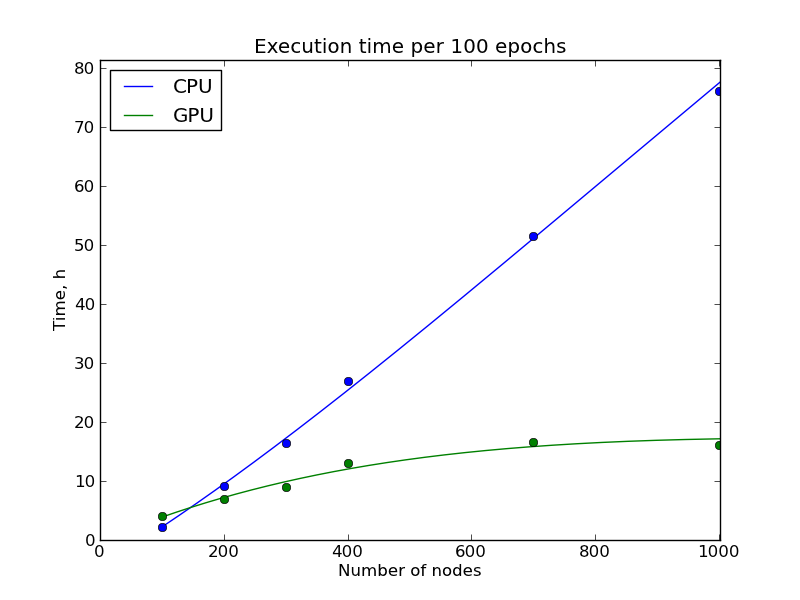
\includegraphics[width=1.0\textwidth]{plots/speedup}
			\caption{Execution time of the GPU algorithm compared to the sequential one}
			\label{fig:speedup}
		\end{minipage}\hfill
		\begin{minipage}[t]{0.45\textwidth}
			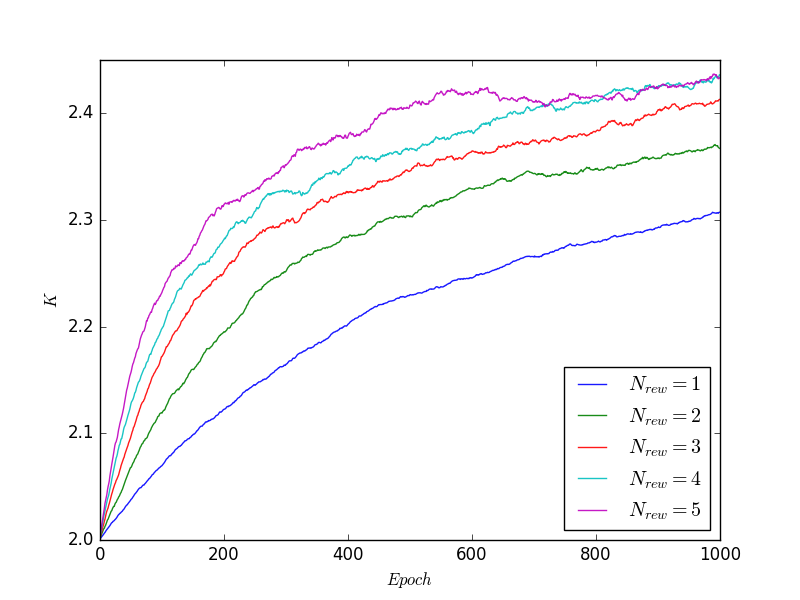
\includegraphics[width=1.0\textwidth]{plots/n_rew}
			\caption{Evolution of mean connectivity for different $N_{rew}$; $N=1000$}
			\label{fig:nrew}
		\end{minipage}
	\end{figure}
	
	\paragraph{Rewiring more than one node per epoch.} In order to determine how $N_{rew}$ influences the rate of convergence to a dynamical equilibrium, we performed $1000$ epochs of evolution with $N=1000$ and $N_{rew}=[1, 5]$. The results of these simulations are shown in Figure \ref{fig:nrew}. With increased value of $N_{rew}$ mean connectivity grows faster and the system reaches steady state at approximately 500th epoch for $N_{rew}=5$. Therefore, we conclude that by rewiring $N_{rew} > 1$ nodes per epoch one can lower the number of epochs required to reach steady state. We limited the attractor length to $\mu_{max}=10^7$ for these experiments.
	
	\paragraph{Limiting the maximum attractor length.} Introducing a limit on attractor length leads to a situation when an attractor can not be found. In these cases $N_{rew}$ nodes are rewired according to their activity during the last $\mu_{max}$ state updates. These states can belong to either a transient period or an attractor. However, the results of our experiments, presented in Tables \ref{table:percentage_of_attractors}, \ref{table:kss}, indicate that low percentage of attractors found does not influence the steady state connectivity obtained as a result of the evolution process.
	
	\begin{table}[ht!]
		\centering
		\begin{tabular}{r | c c c c c}
			& \multicolumn{5}{c}{Nodes count} \\
			$\mu_{max}$	& 100	& 	200	&	300	&	500	&	750\\ \hline
			$5 \cdot 10^4$	&	99.77	&	88.19	&	71.19	&	45.48	&	29.62\\
			$2.5 \cdot 10^5$	&	99.99	&	95.92	&	81.24	&	56.10	&	35.96\\
			$5 \cdot 10^5$	&	100.00	&	97.43	&	86.58	&	59.36	&	38.73\\
			$2.5 \cdot 10^6$	&	100.00	&	99.14	&	92.99	&	68.74	&	46.46\\
			$5 \cdot 10^6$	&	100.00	&	99.53	&	94.40	&	73.00	&	49.22\\
			$1 \cdot 10^7$	&	100.00	&	99.75	&	96.08	&	77.73	&	53.81\\
		\end{tabular}
		\caption{$R$ (percentage of attractors found) for different $N$ and $\mu_{max}$}
		\label{table:percentage_of_attractors}
	\end{table}
	\begin{table}[ht!]
		\centering
		\begin{tabular}{r | c c c c c}
			& \multicolumn{5}{c}{Nodes count} \\
			$\mu_{max}$	& 100	& 	200	&	300	&	500	& 750\\
			\hline
			$5 \cdot 10^4$	&	2.64	&	2.59	&	2.58	&	2.52	&	2.47\\
			$2.5 \cdot 10^5$	&	2.66	&	2.60	&	2.56	&	2.51	&	2.48\\
			$5 \cdot 10^5$	&	2.68	&	2.59	&	2.55	&	2.51	&	2.48\\
			$2.5 \cdot 10^6$	&	2.69	&	2.60	&	2.55	&	2.51	&	2.48\\
			$5 \cdot 10^6$	&	2.69	&	2.59	&	2.55	&	2.52	&	2.48\\
			$1 \cdot 10^7$	&	2.68	&	2.62	&	2.55	&	2.51	&	2.48\\
		\end{tabular}
		\caption{$K_{ss}$ for different $N$ and $\mu_{max}$}
		\label{table:kss}
	\end{table}
	
	Using the approaches discussed above we were able perform simulations on networks consisting of up to 1000 nodes. Plots of the evolution of mean in-degree connectivity and the empirical distribution of attractor lengths are shown in Figures \ref{fig:evolution} and \ref{fig:attractors} respectively. The peaks near $\mu=10^7$ in Figure \ref{fig:attractors} are caused by the limit on the attractor length $\mu_{max} = 10^7$.
	
	
	\begin{figure}[h]
		\begin{minipage}[t]{0.45\textwidth}
			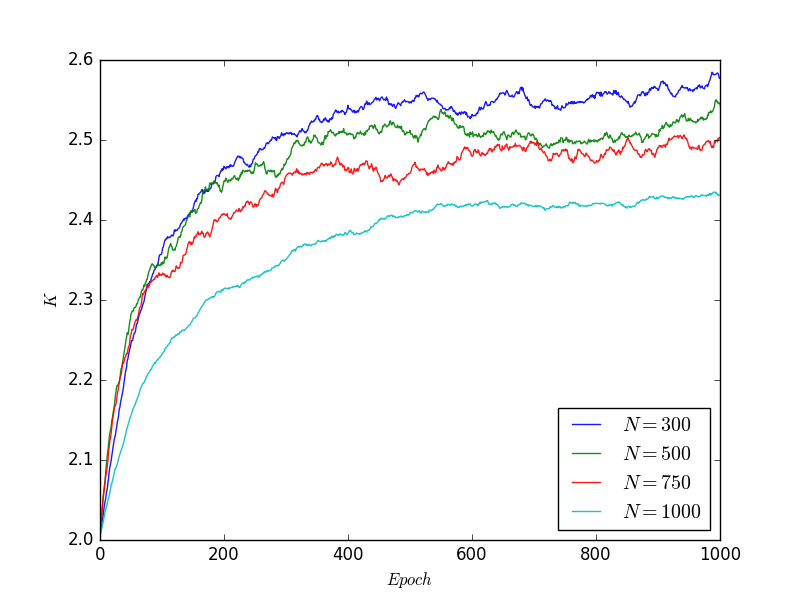
\includegraphics[width=1.0\textwidth]{plots/evolution}
			\caption{Evolution of mean network connectivity}
			\label{fig:evolution}
		\end{minipage}\hfill
		\begin{minipage}[t]{0.45\textwidth}
			\centering
			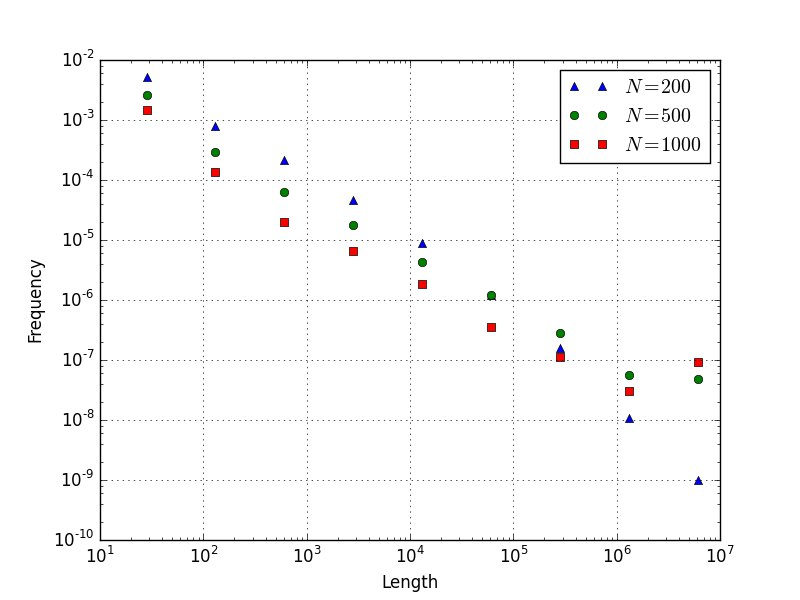
\includegraphics[width=1.0\textwidth]{plots/attractors}
			\caption{Empirical distribution of attractor lengths}
			\label{fig:attractors}
		\end{minipage}
	\end{figure}
	%------------------------------------------------------------------------------
	\clearpage
	\section{Conclusion}
	The enormous size of RBN ensemble makes them appropriate to model various complex systems but also raises significant challenges for their numerical investigation. Even a problem of search for a single attractor of RBN is computationally hard for a networks larger than several dozens of nodes because of an exponential growth of a number of iterations with an increase of a network size.
	
	Finding an attractor for RBN with a given initial state is a basic operation performed for adaptive RBN which change their topology using information about the activity of nodes on the attractor. In this study, we propose a parallel algorithm for GPGPU to speed up simulation of adaptive RBNs which can be used with different sequential algorithms for attractor's search. In addition to updating states for distinct nodes in parallel, we use modified activity-dependent rewiring rule to reduce a number of epochs required for a single run.
	
	Using the algorithm, we performed simulation of networks up to 1000 nodes on a hybrid cluster with NVidia graphic cards. The parallel algorithm demonstrates increasing performance with a growth of a network size (for 1000-nodes network it is approximately 8 times faster than a sequential one). The results show that proposed modification of the rewiring rule allows to reduce a number of epochs to reach a steady state making calculations less time-consumable. We also present the results for a percentage of attractors found for different combinations of sizes of networks and maximum number of iterations examined during search for a single attractor. These values together with the results on mean steady state connectivity can be used for a choice of values of checkpoints in the sequential algorithms of attractor's search.   
	
	\label{sect:conclusion}
	
	%------------------------------------------------------------------------------
	% Refs:
	%
	\label{sect:bib}
	%\bibliographystyle{plain}
	%\bibliographystyle{alpha}
	\bibliographystyle{unsrt}
	%\bibliographystyle{abbrv}
	\bibliography{paper}

\end{document}
